
%(BEGIN_QUESTION)
% Copyright 2010, Tony R. Kuphaldt, released under the Creative Commons Attribution License (v 1.0)
% This means you may do almost anything with this work of mine, so long as you give me proper credit

Suppose a FOUNDATION Fieldbus pressure transmitter is used to measure flow through a process line by sensing differential pressure generated by an orifice plate.  The orifice's rated pressure range is 0 to 100 inches water column, while flowing 0 to 740 liters per minute of liquid.  The operator needs to see the flow rate in units of LPM, and does not care to see or know the differential pressure directly sensed by the transmitter:

$$\includegraphics[width=15.5cm]{i04594x01.eps}$$

Complete the configuration table in the above illustration, showing the proper {\tt XD\_Scale}, {\tt OUT\_Scale}, and {\tt L\_Type} parameter values to make the transmitter function as it should in this application.

\vskip 10pt

Also, determine the direction of flow through this process line, and the proper settings (open or shut) for the three hand valves between the orifice plate and the transmitter while the system is operating normally.

\vskip 20pt \vbox{\hrule \hbox{\strut \vrule{} {\bf Suggestions for Socratic discussion} \vrule} \hrule}

\begin{itemize}
\item{} For those who have studied flow measurement, explain how an orifice plate works to measure fluid flow.
\item{} Suppose the orifice plate is changed for one having a larger bore diameter (i.e. it generates less pressure differential for the same amount of flow).  What, if anything, would have to be re-configured in the FF flow transmitter to accommodate the new orifice plate?
\end{itemize}

\underbar{file i04594}
%(END_QUESTION)





%(BEGIN_ANSWER)

The {\tt L\_Type} parameter needs to be set to ``Indirect Square Root''.

$$\includegraphics[width=15.5cm]{i04594x02.eps}$$

%(END_ANSWER)





%(BEGIN_NOTES)

{\tt XD\_Scale} = 0 to 100 inches water column

\vskip 10pt

{\tt OUT\_Scale} = 0 to 740 LPM

\vskip 10pt

{\tt L\_Type} = Indirect Square Root

\vskip 10pt

Flow direction is right-to-left, based on the ``high'' and ``low'' pressure port orientation on the DP transmitter.


%INDEX% Fieldbus, instrument ranging: setting XD_Scale and OUT_Scale parameters for an application

%(END_NOTES)

